\documentclass[UTF8,12pt, a4paper]{ctexart}

\input{structure.tex}



% \titleformat{\paragraph}
% {\normalfont\normalsize\bfseries}{\theparagraph}{1em}{}
% \titlespacing*{\paragraph}
% {0pt}{3.25ex plus 1ex minus .2ex}{1.5ex plus .2ex}


\begin{document}

\bibliographystyle{plain}

\renewcommand{\contentsname}{Contents}
\renewcommand{\bibname}{reference}

\renewcommand{\today}{\number\year-\number\month-\number\day}

\definecolor{shadecolor}{rgb}{0.92, 0.92, 0.92}

\title{{\vspace{50pt}\Huge TaoQi-doc\linebreak\linebreak}
\vspace{200pt}
}

%please write your name, Student #, and Class # in Authors, student ID, and class # respectively
% \author{\Large 王嘉利 \\}
\author{ %学院\ 计算机学院\\ 姓名\ 王嘉利\\ 学号\ 2018302278\\}
\begin{tabular}{lc}
    学院:& 计算机学院 \\\cline{2-2}
    姓名: & 王嘉利 \\ \cline{2-2}
    学号:& 2018302278 \\\cline{2-2}
    日期:&\today \\ \cline{2-2}
\end{tabular}}

\date{}

\maketitle

\newpage

%----------------------------------------------

\setcounter{secnumdepth}{4}
\tableofcontents
\newpage

\section{背景}

\begin{shaded}
    {\kaishu 这是对将要做的数据库应用简单介绍,以及WISHLIST,此时还未开始开发应用程序。}
\end{shaded}

TaoQi是模仿TaoBao制作的购物平台系统,将采用MySQL和Java开发,使用AndroidStudio作为开发环境。
将采用自顶向下与自地上向混合的方法进行数据库设计。

\textbf{WISHLIST}

\begin{itemize}
    \item \textbf{功能完整性} 
    \item \textbf{并发事务处理正确性} 
    \item \textbf{漂亮的前端设计}
\end{itemize}

\section{需求分析}

在TaoQi应用中,存在三种身份,用户、商家、管理员。

用户在使用应用之前需要先登录。用户可以挑选自己喜欢的商品,加入购物车后下单购买商品。

商家会有自己的商铺,可以在商铺中加入商品。商品将会保存在数据库中。

管理员可以对商品库中的商品进行审核,对用户进行管理等。

将每个部分的综合在一起,得到如下数据流图\autoref{fig:data_flow}。

\begin{figure}[ht]
    \centering
    \includegraphics[width=\textwidth]{./DataFlow.png}
    \caption{数据流图}
    \label{fig:data_flow}
\end{figure}

\section{概念模型}

将上述的数据流图,转化为E-R图。

为了让E-R图比较整洁,这里将主要关心实体之间的联系\autoref{fig:ER}。

\begin{figure}[ht]
    \centering
    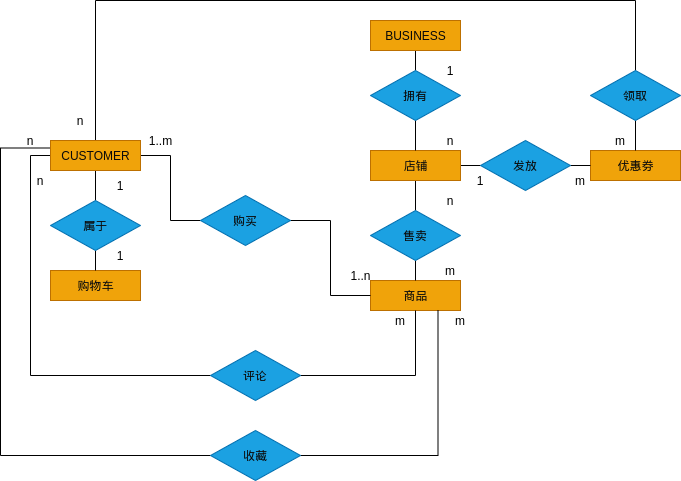
\includegraphics[width=\textwidth]{./ER.png}
    \caption{E-R图  }
    \label{fig:ER}
\end{figure}

将每个实体的属性展开\autoref{fig:ER-detail}。

\begin{figure}[ht]
    \centering
    \includegraphics[width=\textwidth]{./ER-detail.png}
    \caption{实体属性}
    \label{fig:ER-detail}
\end{figure}


%----------------------------------------------

\newpage

\bibliography{ref}



\end{document}
